%	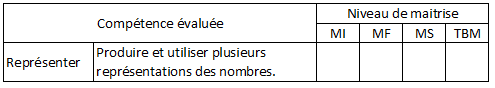
\includegraphics[scale=0.95]{competences}
	
	\section{Calculer}
	
	Calculer astucieusement en détaillant les calculs
	\begin{questions}
		
	
%		\question[2]  $\num{5.5} + 4 + \num{2.5} + 8$
%		\fillwithdottedlines{2cm}
%		%
%		\begin{solution}
%			
%		\end{solution}
			
		
		\question[2]  $\num{3.3} + \num{7.4} + \num{2.7} + \num{2.6} + 8 $
		\fillwithdottedlines{2cm}
		\begin{solution}

		\end{solution}
		
		\question[2]  $\num{3.2} + \num{7.5} + \num{2.8} + \num{5.5} + 15 $
		\fillwithdottedlines{2cm}
		\begin{solution}
			
		\end{solution}
	
	
		\question[2]  $\num{5} \times 25 \times 11 \times \num{4} \times 2$
		\fillwithdottedlines{2cm}
		\begin{solution}
			
		\end{solution}
	
		\question[2]  $\num{2.5} \times 4 \times 3 \times 7$
		\fillwithdottedlines{2cm}
		\begin{solution}
			
		\end{solution}
	
	
		
	
		\question[2]  $\num{12.5} \times 25 \times \num{8} \times 4$
		\fillwithdottedlines{2cm}
		\begin{solution}
			
		\end{solution}
	
	\newpage
	
	
		\question[2]  $\num{5} \times 50  \times \num{4} \times 2$
		\fillwithdottedlines{2cm}
		\begin{solution}
			
		\end{solution}
	
		
	
	
		\question[2]  $\num{3} \times 45 \times 20 \times \num{5} $
		\fillwithdottedlines{2cm}
		\begin{solution}
			
		\end{solution}
	
	
		\question[2]  $(2 + 5) \times (7 + 2) $
		\fillwithdottedlines{2cm}
		\begin{solution}
		
		\end{solution}
	
		\question[2]  $2 + 8 \times 7 + 2 $
		\fillwithdottedlines{2cm}
		\begin{solution}
			
		\end{solution}
	
		\question[2]  $(2 + 8 \times 7) \times 2 $
		\fillwithdottedlines{2cm}
		\begin{solution}
		
		\end{solution}
		
	\end{questions}
	
	
